\chapter{Equivalence of SGD and Frugal-1U}
\label{ch: algo_equal}

\graphicspath{{Figures/Frugal_SGD/}{./}} 

% --------------------------------------------------------------------------------
%                                Quantile Estimation
% --------------------------------------------------------------------------------
           
In 1978, the \textit{pinball loss} function was proposed by \citeauthor{koenkerRegressionQuantiles1978}\cite{koenkerRegressionQuantiles1978}, which is well-known for quantile estimation in both statistics and machine learning. In this chapter, we present the implementation of SGD the approach with the pinball loss function for quantile estimation. We also illustrate that, to some degree, there is an equivalence relationship between our algorithm and the state-of-the-art Frugal-1U\cite{maFrugalStreamingEstimating2014} by both theoretical analysis and experimental results. After the introduction of pinball loss in section~\ref{sec: pinball_loss}, section~\ref{sec: derive_sgd} introduces the SGD methods and at the same time shows the equivalence to Frugal-1U by rephrasing the algorithm. In addition, we offer some complementary explanation, supporting experimental results and further discussion for the proof of algorithm equivalence in section \ref{sec: algo_equivalence}.

\section{Pinball Loss for Quantile Estimation}
\label{sec: pinball_loss}
The pinball function is a convex loss function for estimation of a quantile value.
For a one-dimensional dataset $X = \{x_1, x_2, \cdots, x_N\}$, 
consider the loss function for a single data point $x_i$ $(i \in {1, \cdots, N})$ of the $\tau$-quantile ($\tau \in (0,1)$).
Let $t := x - q$ be the difference between the real value $x$ and the estimate of quantile $q$.
The pinball loss function $\ell_{\tau}(\cdot): \R \to \R_{\geq 0}$ on $t$ is defined by%
%
\begin{equation}
    \ell_\tau(t)= 
        \begin{cases}
            \tau t & t > 0\\
            -(1-\tau) t & t < 0
        \end{cases}
\end{equation}


And the $\tau$-quantile loss has the {\color{black} subgradient}:
% \marginpar{Not sure to use subgradient or gradient and not mention $0$}%
%
\begin{equation}
    \frac {\partial \ell_\tau(t)}{\partial t}= 
        \begin{cases}
            \tau                & t > 0\\
            [\tau, -(1-\tau)]                   & t = 0\\
            -(1-\tau)           & t < 0
        \end{cases}
\end{equation}

Note here we use subgradient instead of gradient, because the pinball loss function is not differentiable at $0$. In the practical implementation of SGD, we choose the the subgradient at $0$ to be $0$. Since the possibility of reaching the $0$ point is $0$, the choice of replacement would not influence the final results. Empirically it is acceptable in this thesis that we ignore the breaking point at $0$ and take this subgradient function as the gradient of pinball loss function.

The overall loss for distribution $X$ with quantile estimation $q$ is%
%
\begin{equation}
    L_{\tau}(q) = \sum_{x \in X} \ell_{\tau}(x - q)
\end{equation}


The best estimate of the $\tau$-quantile $q$ is the $q$ with minimal overall loss. 
Let $q^\ast$ be the best estimate, then we have
\begin{equation}
    q^\ast = \argmin_{q} L_{\tau}(q)
\end{equation}



% --------------------------------------------------------------------------------
%                                SGD for Quantile Estimation
% --------------------------------------------------------------------------------
\section{Deriving the SGD approach from Frugal}
\label{sec: derive_sgd}
Inspired by Frugal-1U\cite{maFrugalStreamingEstimating2014}, we propose a quantile estimation method using the SGD approach with implementation of the pinball loss. Here this algorithm is introduced by rephrasing Frugal-1U, which also provides an intuition for the equivalence of the two algorithms.

\subsection{Pseudo Code for the Frugal-1U Algorithm}

As a quantile estimation algorithm using constant memory storage, Frugal-1U reaches the extreme minimum of memory usage, as it "uses only one unit of memory per group to compute a quantile for each group"\cite{maFrugalStreamingEstimating2014}. Besides the minimal memory usage, the update method is also computationally simple. The pseudo-code of Frugal-1U is presented as algorithm~\ref{alg:frugal_1U}.
% \marginpar{the pseudo code has already been mentioned in literature review}
\begin{algorithm}
\caption{Frugal-1U}\label{alg:frugal_1U}
    \begin{algorithmic}[1]
        \Require{Data Stream $X$, $k$, $Q$, $1$ unit of memory $q$}
        \Ensure{$q$}
        % \Procedure{frugal}{$X,\tau$}            \Comment{X is the dataset}
        \State {Initialization $q = 0$}               %\Comment{Default initialization $q_0$ = 0}
            \For{\textbf{each} $x_i$ in $X$}                  %\Comment{Parameter update for each input data point}
                \State{$rand$ = random(0,1)}
                \Comment{get a random value in $[0,1]$}
                % \State {\textbf{set} $\alpha_k$} \Comment{Set step size}
                \If{$x_i > q$ \textbf{and} $rand > 1-\frac{k}{Q}$} %\Comment{$q_{k+1} = q_k + \alpha_k \tau$ when $x_k - q_k > 0$}
                    \State{$q = q + 1$;}
                \Else { \textbf{if} $x_i < q$ \textbf{and} $rand > \frac{k}{Q}$}  %\Comment{$q_{k+1} = q_k - \alpha_k (1-\tau)$ otherwise}
                    \State{$q = q - 1$;}
                \EndIf
            \State{\textbf{end if}}
            \EndFor
        \State{\textbf{end for}}
        % \State \textbf{return} $q$              \Comment{$q_k$ is the SGD result of quantile estimate}
        % \EndProcedure
    \end{algorithmic}
\end{algorithm}

The output $q$ is the estimate of the $k$th $Q$-quantile (see section \ref{subsec: quant}) for a given data stream $X$. 
By rephrasing of some steps of Frugal-1U, 
its equivalence to an SGD algorithm for quantile estimation will be shown in the following part.
\\\\
\textbf{Rephrasing of the Algorithm} \label{replacements}
% \marginpar{this should be removed, just change the notations}
\begin{enumerate}
    \item The constant $\frac{h}{k}$ is replaced by $\tau$, since the $\tau$-quantile is defined
     as the $h$th $k$-quantile point in chapter \ref{ch: intro}.
    % \item The quantile estimate $\tilde{m}$ is replaced by $q$, as it stands for estimate of quantile.
    \item The generation of the random number and it's comparison with $1-\frac{h}{k}$ or $\frac{h}{k}$
    in line 3 to 7 is replaced by the following algorithm.
    \begin{algorithm}
        \begin{algorithmic}[1]
            \setcounter{ALG@line}{2}
            \State{ }   \Comment{No need to generate a random number}
            \If{$x_i > q$} %\Comment{$q_{k+1} = q_k + \alpha_k \tau$ when $x_k - q_k > 0$}
                \State{$q = q + 1 \times (1-\frac{h}{k})$}     
                \Comment{$P((rand > 1-\frac{h}{k}) \mid rand \in \mathcal{U}(0,1)) = 1-\frac{h}{k}$;}
            \Else { \textbf{if} $x_i < q$}  %\Comment{$q_{k+1} = q_k - \alpha_k (1-\tau)$ otherwise}
                \State{$q = q - 1 \times \frac{h}{k}$}         
                \Comment{$P((rand > \frac{h}{k}) \mid rand \in \mathcal{U}(0,1)) = \frac{h}{k}$;}
            \EndIf 
        \end{algorithmic}
    \end{algorithm}

    % Here the probability $P((rand > p) \mid rand \in \mathcal{U}(0,1))$ is the simplification
    % for the generation of random number $rand$ and it's comparison to a constant $p$ $(0 < p < 1)$.
    
    To understand this replacement, consider the 3 steps:
    \begin{enumerate}[label={(\roman*)}]
    \item generate a random number $rand$, 
    \item compare it with a constant $p$, and
    \item take action if $rand > p$. 
    \end{enumerate}
    This can be interpreted as ``take the action with probability 
    $P((rand > p) \mid rand \in \mathcal{U}(0,1))$''. 

    While the behaviour is different, this replacement preserves the expected change of $q$. 
    For example when $x_i > q$, 
    the expected change of $q$ is
    $E_1[\nabla q] = E[q \times p]$ in the Frugal-1U with 
    random number generation,
    while 
    $E_2[\nabla q] = q \times p$ in the replacement method.
    Since $E_1[\nabla q] = E_2[\nabla q]$, the replacement is valid
    with regard to the expectation of the change in quantile estimate during each step.

\end{enumerate}


\subsection{SGD for pinball loss function}
% \marginpar{change $q_k$ to $q_i$}
Let $q_0$ be the initial guess of the quantile estimate. 
By SGD, the estimate is updated each step with a data point from the distribution.
\begin{equation}
    q_{k+1} = q_k - \alpha_k g_k
\end{equation}

where $ \alpha_k $ is a suitable step size and 

\begin{equation}
    g_k = \partial L_{\tau}^{(k)}(q_k) \in \frac{\partial l_\tau(x_k - q_k)}{\partial q_k}
\end{equation}
{Notice here partial is taken because the gradient of a single variable function equals the partial of it.}
\\\\
Then we have
\begin{equation*}
    q_{k+1} = 
    \begin{cases}
        q_k + \alpha_k \tau               & x_k - q_k > 0\\
        q_k                               & x_k - q_k = 0         \\
        q_k - \alpha_k (1-\tau)           & x_k - q_k < 0\\
        % [\tau, -(1 - \tau)] & t = 0
    \end{cases}
\end{equation*}

% \marginpar{
% {\color{red} \textbf{Problem}}
% In Frugal-1U the quantile estimate $q$ does not change when $x_k = q$, but in SGD 
% % the quantile estimate is updated: $q = q-\alpha_k (1-\tau)$. This can be seen as different
% } 
\begin{algorithm}
    \caption{SGD algorithm}\label{alg:SGD}
    \begin{algorithmic}[1]
        \Require{Data Stream $X$, $\tau$, $1$ unit of memory $q$}
        \Ensure{$q$}
        % \Procedure{frugal}{$X,\tau$}            \Comment{X is the dataset}
        \State {Initialize} $q$                 \Comment{Default initialization $q_0$ = 0}
            \For{$x_k$ in $X$}                  \Comment{Parameter update for each input data point}
                \State \textbf{set} $\alpha_k = 1$  \Comment{Set step size}
                \If{$x_k > q$}                  \Comment{$q_{k+1} = q_k + \alpha_k \tau$ when $x_k - q_k > 0$}
                    \State{$q = q + \alpha_k \tau$}
                \Else                           \Comment{$q_{k+1} = q_k - \alpha_k (1-\tau)$ otherwise}
                    \State{$q = q - \alpha_k (1-\tau)$}
                \EndIf
            \EndFor
        \State \textbf{return} $q$              \Comment{$q_k$ is the SGD result of quantile estimate}
        % \EndProcedure
    \end{algorithmic}
\end{algorithm}
Besides the replacements mentioned in section \ref{replacements}, the notation has changed from Frugal-1U to SGD: 
$X$ is used instead of $S$ for the data stream. The other important change is the introduction of step size. Specifically, the step size $\alpha$ is not mentioned in Frugal-1U because it is fixed as constant $1$. On the other hand, the choice of constant or variable step size $\alpha_i$ is an important feature of the SGD algorithm. The flexibility of step size can contribute to a better convergence rate when appropriate step sizes are chosen.


% \textbf{subgradient} values for $l_\tau(x_k - q_k)$ 
% {\color{red} \textbf{but then I need to explain subgradient descent}} 
% --------------------------------------------------------------------------------
%                              Equality of two algorithms 
% --------------------------------------------------------------------------------
\section{Equivalence of Algorithms}
\label{sec: algo_equivalence}

The derivation of the SGD algorithm from Frugal-1U has intuitively shown the evident similarity between them. In this section, we investigate the similarity between our approach, which we refer to as the SGD algorithm, and Frugal-1U, which leads to the proof of equivalence by experimental performances with additional discussion.

\subsection{Comparison experiments between SGD and Frugal-1U}

We investigate various aspects of the similarity between the SGD algorithm and the Frugal-1U algorithm: behaviours and results on different data distributions. The behavioural similarity is inspired by the \textit{behavioural equivalence} \cite{gurevichSequentialAbstractstateMachines2000}, which requires sequential algorithms to have same states, same initial states, and the same transition function when converted to an abstract state machine (ASM). The quantile estimation results are compared based on the final output results of the algorithms.

\subsubsection{Data distributions and algorithm settings}
\label{subsubsec: distro_and_setting}
For comprehensiveness, we evaluate the algorithms using data generated from three distributions:
    \begin{enumerate}
        \item a Gaussian distribution with mean 2 and standard derivation 18 (\textit{gau-1})
        \item a mixed Gaussian distribution composed of 5 Gaussian distributions (\textit{mix}):
            \begin{enumerate}
                \item weight = 0.3, mean = 2, standard derivation = 7
                \item weight = 0.2, mean = 0, standard derivation = 0.7
                \item weight = 0.1, mean = 36, standard derivation = 26
                \item weight = 0.15, mean = 5, standard derivation = 77
                \item weight = 0.25, mean = -77, standard derivation = 7
            \end{enumerate}
            \item a exponential distribution of rate 1, and is scaled by $6.5$ and shifted by $-20$
    \end{enumerate}
The algorithms are initialised with the starting estimate for any quantile value at $0$. The step size of the SGD algorithm is set as constant 1 to match the implicit step size of Frugal-1U. Each data stream contains 1000 randomly ordered samples from the corresponding distribution with a fixed sequence. The estimation on the $0.1, 0.3, 0.5, 0.9,$ and $0.99$ quantiles are checked.

\subsubsection{Evaluation methods}

For each simulation setup, we run the Frugal-1U algorithm 100 times and SGD once. Since the data stream is a fixed sequence of data points, the behaviour and result of SGD are also fixed, whereas Frugal-1U is likely to perform differently given its randomness in each update step. For a quantile probability $\tau$, let $\tau$-$q_{\text{batch}}$ be the computation results of the batch quantile, $\tau$-$q_{\text{SGD}}$ and $\tau$-$q_{\text{frugal}}$ be the results respectively of SGD and Frugal-1U algorithm. The similarity of the two estimates $S_\tau$ is measured by
\begin{equation}
    S_\tau = \frac{ \tau\text{-}q_{\text{SGD}} - \tau\text{-}q_{\text{frugal}} }{ \tau\text{-}q_{\text{SGD}} - \tau\text{-}q_{\text{batch}} }
    \label{eq: frugal_err}
\end{equation}
where a smaller $|S_\tau|$ means a higher similarity, and $|S_\tau| = 0$ means the two quantile estimates are the same. In this paper, we consider $\leq 2^6 = 64$ as the threshold for the similarity error, that is, if $|S_\tau| \leq 2^6$, we believe the the two results are similar enough to be viewed as "equal".

Both algorithms start the quantile estimate at $0$. When a new observation arrives, Frugal-1U updates the value by $1$ or $0$ according to probability, while the update is a deterministic floating number for SGD. The behavioural similarity is compared at each update step. For Frugal-1U, we take the mean value of the quantile estimate update over 100 runs, and it is compared with the one fixed SGD value at the same epoch. 

\subsubsection{Results for similarity comparisons}

The mechanism for data generation is as follows. First, generate a dataset with 1000 samples according to one of the three distributions specified in section~\ref{subsubsec: distro_and_setting}. For each distribution, we also compute the true quantiles. The sequence of the dataset is fixed for all the experiments, including one computation for the batch quantiles, one for the SGD quantiles, and 100 for the Frugal-1U quantiles. The process of quantile estimation is shown in the process plots (fig \ref{fig: gau_1_proc_explanation}, \ref{fig: mix_proc}, and \ref{fig: exp_proc}), in which we can see the comparison in algorithm behaviours. The true quantiles are also shown in these plots, as a reference to the algorithm performances.
Figure \ref{fig: gau_1_err_explanation}, \ref{fig: mix_err}, and \ref{fig: exp_err} show the similarity error values of the final results only.

It is also worthwhile to point out that while 1000 is not a large size for data streams, it is sufficient to evaluate the similarity between the two algorithms as it does not need to show the convergence to the true quantile. In fact, the convergence of most quantile probabilities over the three datasets are already reached by the 1000 epochs.

The process plot in fig \ref{fig: gau_1_proc_explanation} comparing Frugal-1U and SGD shows that the mean of Frugal-1U steps and the SGD functions are largely overlapped. Take the $0.1$-quantile for example, the two algorithms start at the same point, and the mean Frugal-1U line shares similar trends and close quantile estimate position with SGD. They even overlap in many intervals (where the dark blue line is covered by the light blue line).
Irrespective of the data distribution and the quantile probabilities, it is clearly shown in figure \ref{fig: gau_1_proc_explanation}, \ref{fig: mix_proc}, and \ref{fig: exp_proc} that the quantile estimation behaviours of mean Frugal-1U and SGD are very similar. However, this evidence is not sufficient to claim a close similarity because the randomness of Frugal-1U might lead to a large variety in behaviours.

For a closer examination, the similarity error values of the quantiles are checked at the result states. Figure \ref{fig: gau_1_err_explanation} illustrates the distributions of similarity error values between the 100 runs of Frugal-1U and the one SGD result on \textit{gau-1}. Take the $0.1$-quantile for example, the similarity error values are distributed in the range $(-2^4, 2^3)$, which means $|S_\tau| < 2^6$ for all 100 runs. Furthermore, the mean of the similarity error (the vertical black line) has an absolute value less than 1, indicating the mean Frugal-1U result and the SGD result is nearly the same. The results from the three figures (fig \ref{fig: gau_1_err_explanation}, \ref{fig: mix_err}, and \ref{fig: exp_err}) also imply the high similarity of Frugal-1U and SGD works for all three distributions and all five quantiles checked in the experiment.

Results from the experiments (fig \ref{fig: gau_1_proc_explanation} to \ref{fig: exp_err}) support our theoretical conjecture that the two algorithms are highly similar in both behaviours and results regardless of distributions or quantile probability values. The similarity is high enough to meet our requirement for the equivalence (absolute similarity error value less than or equal to 64).

% \marginpar{I think more data is required, for example the mean and variance comparison on processes?}

\begin{figure}[h!]
    \centering
    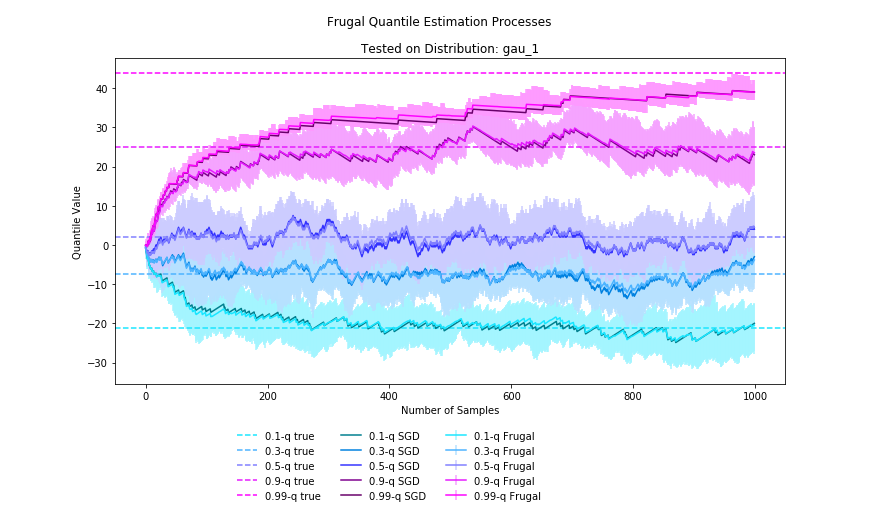
\includegraphics[width=1\columnwidth]{gau_1_proc.png}
    \caption{Quantile estimation behaviour similarity between Frugal-1U and SGD on the \textit{gau-1} dataset. The horizontal dotted lines are the true quantiles, the dark solid colour lines are SGD quantiles, and the lighter solid colour lines are the mean value of Frugal-1U quantiles. The light coloured shadows around the solid lines are the range of Frugal-1U steps over the 100 runs. For each epoch, the top and the bottom margin of the shadow are positioned respectively on the maximum and minimum value of the 100 experiments. The shadow of a quantile is an indicator of how much the Frugal-1U estimate varies around the mean value. Unfortunately the shadows from different quantiles sometimes cover each other, so the it can only be used as a rough visual reference of changes in Frugal-1U.}
    \label{fig: gau_1_proc_explanation}
\end{figure}

\begin{figure}[h!]
    \centering
	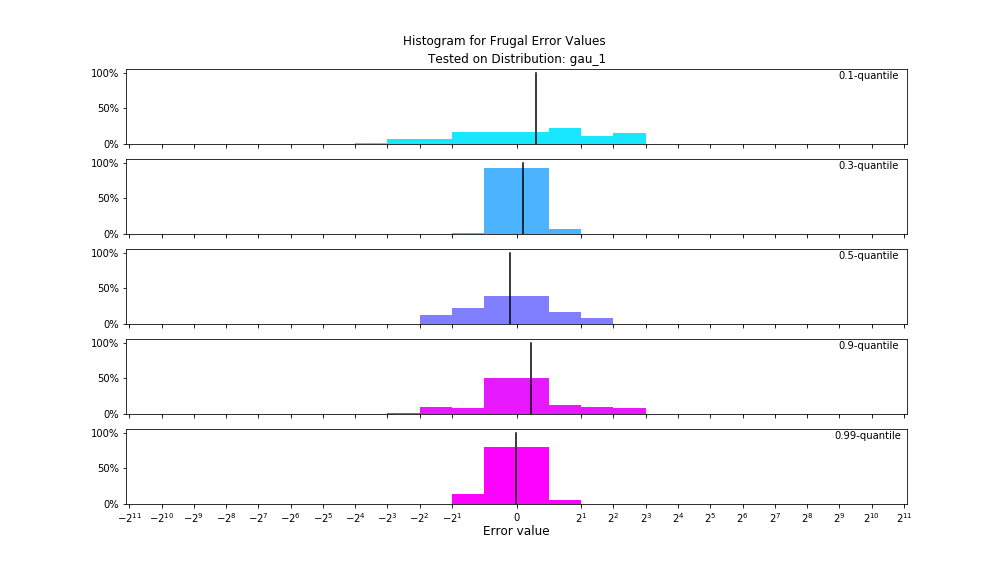
\includegraphics[width=1\columnwidth]{gau_1_err.png}
    \caption{Quantile estimation result similarity between Frugal-1U and SGD on the \textit{gau-1} dataset.
    Each of the 5 histograms represents the distribution of Frugal-1U similarity error values for a specific quantile. The similarity error values are compared by function \eqref{eq: frugal_err}. For example, consider the top one (the $0.1$-quantile). The distribution of 100 similarity error values are shown in the bright blue histogram. The mean similarity error value is also in the form of the vertical black line.}
    \label{fig: gau_1_err_explanation}
\end{figure}

\begin{figure}[h!]
    \centering
	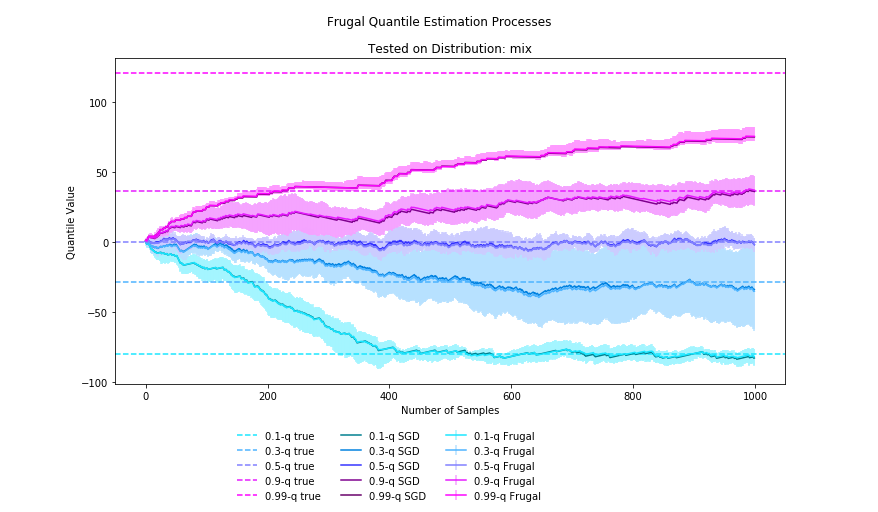
\includegraphics[width=1\columnwidth]{mix_proc.png}
    \caption{Quantile estimation behaviour similarity between Frugal-1U and SGD on the \textit{mix} dataset}
    \label{fig: mix_proc}
\end{figure}

\begin{figure}[h!]
    \centering
	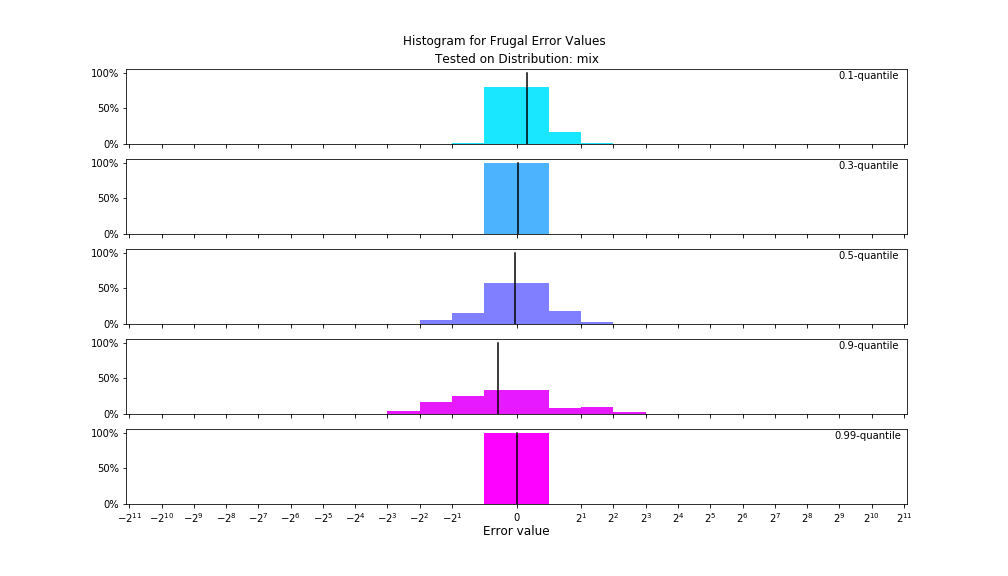
\includegraphics[width=1\columnwidth]{mix_err.png}
    \caption{Quantile estimation result similarity between Frugal-1U and SGD on the \textit{mix} dataset}
    \label{fig: mix_err}
\end{figure}

\begin{figure}[h!]
    \centering
	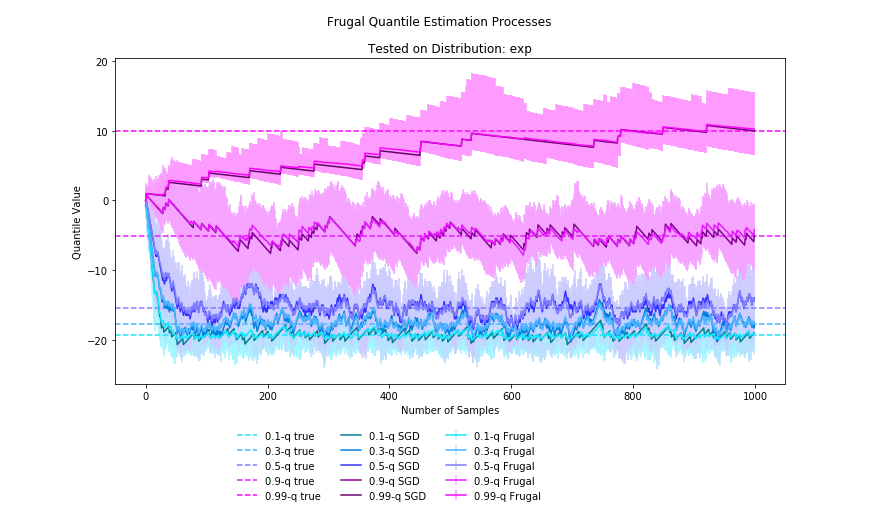
\includegraphics[width=1\columnwidth]{exp_proc.png}
    \caption{Quantile estimation behaviour similarity between Frugal-1U and SGD on the \textit{exp} dataset}
    \label{fig: exp_proc}
\end{figure}

\begin{figure}[h!]
    \centering
	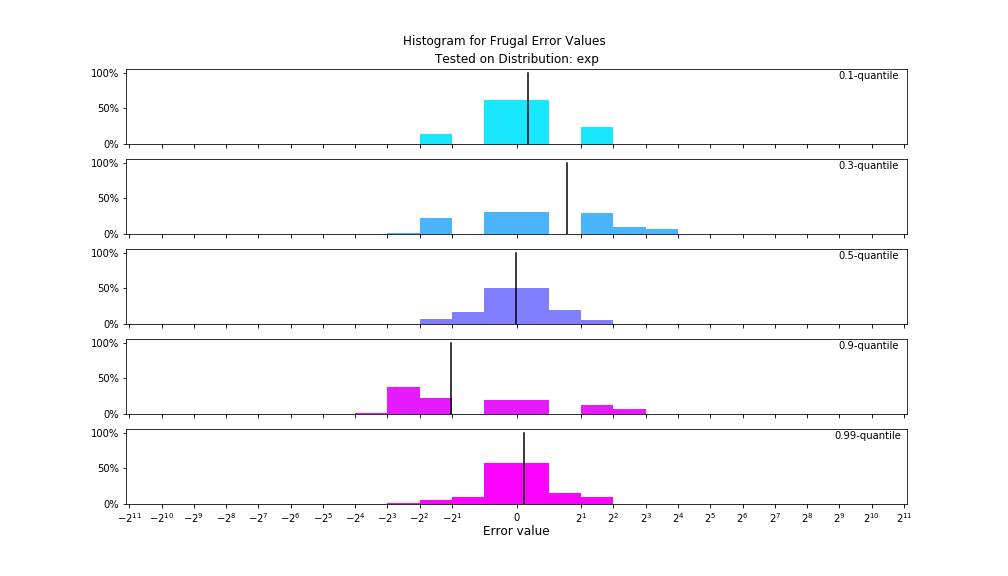
\includegraphics[width=1\columnwidth]{exp_err.png}
    \caption{Quantile estimation result similarity between Frugal-1U and SGD on the \textit{exp} dataset}
    \label{fig: exp_err}
\end{figure}

\subsection{Discussion about the equivalence}

The comparison experiments between Frugal-1U and SGD implies there is a high similarity relation between them with regards to both behaviours and results.
Although it is claimed in this paper that the SGD algorithm and the Frugal-1U algorithm are equivalent to some extent, \citeauthor{blassWhenAreTwo2008}\cite{blassWhenAreTwo2008} have already pointed out that there is no such relation as equivalence between any two algorithms. 

 The claim that the two algorithms are equivalent is based on the check of similarity error value. It is obvious that if the requirement for similarity error value is more strict, e.g. $|S_\tau| \leq 2^2$, then the equivalence would no longer hold for some distribution and quantile value settings. That is what we refer to as "equivalence to some extent".

\section{Conclusion}
The SGD algorithm is proposed by derivation from the Frugal-1U algorithm. We performed an empirical comparison between Frugal-1U and SGD over 3 different distributions. In addition, we had a theoretical discussion about the equivalence between them. The two algorithms are shown to be equal to some extent. As Frugal-1U is a valid quantile estimation method, we deduce that SGD is a valid quantile estimation method by equivalence.
The main difference is that SGD is overall more stable than Frugal-1U.
Although SGD is not random for a fixed sequence data stream, it benefits in flexibility in the form of an adjustable step size.
In the next chapter we investigate various settings of SGD in more detail.